%=========== ΛΥΣΗ - 4ο ΘΕΜΑ Δ ===========
\begin{thema}{Δ}
Η συνάρτηση $f$ έχει πεδίο ορισμού το $\mathbb{R}$, αφού
\[
x^2+1>0
\]
για κάθε $x\in\mathbb{R}$.
\begin{erwthma}
\item Για τις ασύμπτωτες της $C_f$ έχουμε
\[
\lim_{x\to\pm\infty}f(x)
=\lim_{x\to\pm\infty}\frac{x^2}{x^2+1}
=\lim_{x\to\pm\infty}\frac{1}{1+\frac{1}{x^2}}
=1.
\]
Επομένως η ευθεία
\[
{y=1}
\]
είναι οριζόντια ασύμπτωτη της $C_f$ τόσο στο $+\infty$ όσο και στο $-\infty$. Η $C_f$ δεν έχει κατακόρυφες ασύμπτωτες, διότι $x^2+1\neq0$ για κάθε $x\in\mathbb{R}$, ούτε πλάγιες ασύμπτωτες, αφού έχει οριζόντια ασύμπτωτη.

Η $f$ είναι παραγωγίσιμη στο $\mathbb{R}$ και
\[
f'(x)
=\frac{2x(x^2+1)-x^2\cdot2x}{(x^2+1)^2}
=\frac{2x}{(x^2+1)^2}.
\]
Επειδή $(x^2+1)^2>0$ για κάθε $x\in\mathbb{R}$, το πρόσημο της $f'$ είναι το πρόσημο του $x$. Επομένως:
\begin{itemize}
\item $f'(x)<0$ για $x<0$,
\item $f'(0)=0$,
\item $f'(x)>0$ για $x>0$.
\end{itemize}
Στον παρακάτω πίνακα βλέπουμε το πρόσημο της $f'$ και τη μονοτονία της $f$:
\begin{center}
\begin{tikzpicture}
\tkzTabInit[color,lgt=2,espcl=1.8,colorC = maincolor!50!white,colorL = maincolor!20!white,colorV = maincolor!50!white]%
{$x$ / .8,$f'(x)$ /0.8,$f(x)$/0.8}%
{$-\infty$,$0$,$+\infty$}%
\tkzTabLine{, -, z, +, }
\tkzTabVar{+/{1},-/{0},+/{1}}
\end{tikzpicture}
\end{center}

Άρα η $f$ είναι \textbf{γνησίως φθίνουσα} στο $(-\infty,0]$ και \textbf{γνησίως αύξουσα} στο $[0,+\infty)$. Παρουσιάζει ολικό ελάχιστο στο $x_0=0$, με τιμή
\[
f(0)=0.
\]
Επίσης, για κάθε $x\in\mathbb{R}$,
\[
f(x)=\frac{x^2}{x^2+1}<1.
\]
Συνεπώς το σύνολο τιμών της $f$ είναι
\[
{f(\mathbb{R})=[0,1)}.
\]

\item Για κάθε $x\in\mathbb{R}$ είναι
\begin{align*}
f''(x)
&=\left[\frac{2x}{(x^2+1)^2}\right]'\\
&=\frac{2(x^2+1)^2-2x\cdot2(x^2+1)\cdot2x}{(x^2+1)^4}\\
&=\frac{2(x^2+1)-8x^2}{(x^2+1)^3}\\
&=\frac{2(1-3x^2)}{(x^2+1)^3}.
\end{align*}
Επειδή $(x^2+1)^3>0$, το πρόσημο της $f''$ είναι το πρόσημο της παράστασης $1-3x^2$. Έχουμε
\[
f''(x)=0
\Leftrightarrow 1-3x^2=0
\Leftrightarrow x=\pm\frac{1}{\sqrt{3}}.
\]
Επιπλέον:
\begin{itemize}
\item $f''(x)>0$ για $-\frac{1}{\sqrt{3}}<x<\frac{1}{\sqrt{3}}$,
\item $f''(x)<0$ για $x<-\frac{1}{\sqrt{3}}$ ή $x>\frac{1}{\sqrt{3}}$.
\end{itemize}
Στον παρακάτω πίνακα βλέπουμε το πρόσημο της $f''$ και την κυρτότητα της $f$:
\begin{center}
\begin{tikzpicture}
\tkzTabInit[color,lgt=2,espcl=1.5,colorC = maincolor!50!white,colorL = maincolor!20!white,colorV = maincolor!50!white]%
{$x$ / .8,$f''(x)$ /0.8,$f(x)$/0.8}%
{$-\infty$,$-\frac{1}{\sqrt{3}}$,$\frac{1}{\sqrt{3}}$,$+\infty$}%
\tkzTabLine{, -, z, +, z, -, }
\tkzTabLine{,\curvearrowright,t,\rotatebox[origin=c]{180}{$\curvearrowleft$},t,\curvearrowright,}
\end{tikzpicture}
\end{center}

Άρα η $f$ είναι \textbf{κυρτή} στο $\left[-\frac{1}{\sqrt{3}},\frac{1}{\sqrt{3}}\right]$ και \textbf{κοίλη} στα διαστήματα $\left(-\infty,-\frac{1}{\sqrt{3}}\right]$ και $\left[\frac{1}{\sqrt{3}},+\infty\right)$.

Επειδή η $f''$ αλλάζει πρόσημο στα $x=\pm\frac{1}{\sqrt{3}}$, η $C_f$ έχει σημεία καμπής τα
\[
K_1\left(-\frac{1}{\sqrt{3}},\frac{1}{4}\right)
\quad\text{και}\quad
K_2\left(\frac{1}{\sqrt{3}},\frac{1}{4}\right),
\]
αφού
\[
f\left(\pm\frac{1}{\sqrt{3}}\right)
=\frac{\frac{1}{3}}{\frac{1}{3}+1}
=\frac{1}{4}.
\]

\item Για κάθε $x\neq0$ έχουμε
\begin{align*}
f\left(\frac{1}{x}\right)
&=\frac{\frac{1}{x^2}}{\frac{1}{x^2}+1}
=\frac{1}{x^2+1}.
\end{align*}
Επομένως
\[
f(x)+f\left(\frac{1}{x}\right)
=\frac{x^2}{x^2+1}+\frac{1}{x^2+1}
=1.
\]

Η συνάρτηση $g(x)=f(e^x)-\frac{1}{2}$ έχει πεδίο ορισμού το $\mathbb{R}$. Για κάθε $x\in\mathbb{R}$ είναι
\begin{align*}
g(-x)
&=f(e^{-x})-\frac{1}{2}\\
&=f\left(\frac{1}{e^x}\right)-\frac{1}{2}\\
&=1-f(e^x)-\frac{1}{2}\\
&=-\left(f(e^x)-\frac{1}{2}\right)\\
&=-g(x).
\end{align*}
Άρα η $g$ είναι \textbf{περιττή}.

\item Θέτουμε
\[
I=\int_{1/a}^{a}f(x)\d x,\quad a>1.
\]
Χωρίζουμε το ολοκλήρωμα στο σημείο $1$:
\[
I=\int_{1/a}^{1}f(x)\d x+\int_1^a f(x)\d x.
\]
Στο πρώτο ολοκλήρωμα θέτουμε
\[
x=\frac{1}{t},
\quad
\d x=-\frac{1}{t^2}\d t.
\]
Για $x=\frac{1}{a}$ είναι $t=a$, ενώ για $x=1$ είναι $t=1$. Επομένως
\begin{align*}
\int_{1/a}^{1}f(x)\d x
&=\int_a^1 f\left(\frac{1}{t}\right)\left(-\frac{1}{t^2}\right)\d t\\
&=\int_1^a\frac{f\left(\frac{1}{t}\right)}{t^2}\d t\\
&=\int_1^a\frac{1-f(t)}{t^2}\d t.
\end{align*}
Άρα
\begin{align*}
I
&=\int_1^a\left[\frac{1-f(x)}{x^2}+f(x)\right]\d x\\
&=\int_1^a\left[\frac{1}{x^2(x^2+1)}+\frac{x^2}{x^2+1}\right]\d x\\
&=\int_1^a\left(1+\frac{1}{x^2}-\frac{2}{x^2+1}\right)\d x\\
&=\left[x-\frac{1}{x}-2\arctan x\right]_1^a\\
&=a-\frac{1}{a}-2\arctan a+\frac{\pi}{2}.
\end{align*}
Επομένως
\[
{\int_{1/a}^{a}f(x)\d x
=a-\frac{1}{a}-2\arctan a+\frac{\pi}{2}},
\quad a>1.
\]
\end{erwthma}
\end{thema}
%=========== ΤΕΛΟΣ ΛΥΣΗΣ - 4ο ΘΕΜΑ Δ ===========
